%-------------------------------------------------------------------------------
%                            BAB II
%               TINJAUAN PUSTAKA DAN DASAR TEORI
%-------------------------------------------------------------------------------

\chapter{TINJAUAN PUSTAKA DAN DASAR TEORI}                

\section{Tinjauan Pustaka}
  Secara umum, cara untuk menghubungkan \emph{Wireless Sensor Network} (WSN) dengan jaringan internet dapat dikelompokkan menjadi dua \cite{Rodrigues2010}. Cara pertama adalah menggunakan \emph{gateway} \cite{DaSilvaCampos2011} dan cara yang kedua adalah dengan menggunakan simpul sensor yang sudah dilengkapi dengan protokol internet. Cara yang lebih mudah ditempuh adalah dengan cara yang pertama karena pengubahan yang dilakukan relatif tidak terlalu besar. Sedangkan cara yang kedua akan menemui banyak kendala terutama pada WSN yang sudah terpasang karena harus dilakukan penggantian tiap simpul sensor.

  Salah satu usaha untuk mengintegrasikan jaringan WSN dengan jaringan WiFi menggunakan \emph{gateway} misalnya dilakukan pada penelitian yang dilakukan oleh \cite{Spinar2009}. Pada penelitian tersebut pengintegrasian dilakukan dengan sebuah komputer yang didedikasikan untuk keperluan tertentu. Penggunaan komputer khusus ini adalah \emph{hardware-solution} yang membutuhkan biaya dan kerumitan sistem.

  Riset \cite{Dunkels2004} juga menawarkan pengintegrasian dengan jaringan berbasis \emph{Internet Protocol} (IP). Namun demikian di dalam riset ini diperlukan pengubahan yang signifikan jika konfigurasi jaringan sensor nirkabel sudah terpasang. Simpul sensor yang digunakan harus diganti dengan simpul sensor yang mendukung IP. Hal ini jelas akan memakan biaya yang cukup besar dan tidak praktis untuk dilakukan. Terlebih lagi jika jumlah sensor yang telah terpasang jumlahnya cukup banyak.

  Penelitian \cite{wibowo2013wireless} sudah berhasil mengembangkan sebuah \emph{Access Point} (AP) menjadi \emph{gateway} yang dapat digunakan untuk menghubungkan sebuah protokol WSN dengan jaringan IP. Protokol WSN yang digunakan adalah protokol dari IQRF. Penelitian tersebut kemudian dilanjutkan dengan penelitian \cite{widyawan2012ihome} yang sudah diterapkan dalam sistem \emph{domotic}.

  Penelitian ini merupakan kelanjutan dari penelitian yang telah dikembangkan oleh \cite{wibowo2013wireless} dan \cite{widyawan2012ihome}. Pada penelitian tersebut, belum ada interoperabilitas berbagai \emph{vendor} ke dalam sebuah AP. Oleh karena itu, penelitian ini berusaha untuk, selain menginteroperabilitaskan WSN dan IP, juga mengintegrasikan dua jenis WSN ke dalam sebuah AP untuk meningkatkan sisi interoperabilitas. Selain itu, penelitian ini juga mengembangkan antarmuka berbasis web yang responsif, yang akan beradaptasi dengan ukuran layar secara otomatis, sehingga pengendalian WSN dapat dilakukan dari komputer hingga ponsel cerdas.

\section{Landasan Teori}
  \subsection{\emph{Wireless Sensor Network}}
    Jaringan sensor nirkabel, atau yang juga dikenal dengan \emph{Wireless Sensor Network}, adalah jaringan simpul sensor otonom yang terdistribusi digunakan untuk memonitor kondisi fisik atau lingkungan \cite{Erratt2013} misalnya suhu, suara, getaran, kelembaban, dan lain-lain. Selain itu, tidak menutup kemungkinan untuk menambahkan fungsi tambahan pada setiap simpul misalnya port masukan/keluaran (I/O port) yang terdapat dalam setiap simpul dihubungkan dengan aktuator sehingga dapat digunakan untuk mengendalikan piranti elektrik atau elektronis.

    Secara umum, WSN dapat diilustrasikan seperti Gambar \ref{wsn}. Pada gambar tersebut terlihat adanya beberapa simpul yang diwakili dengan titik berukuran kecil dan satu buah simpul yang diwakili dengan titik berukuran lebih besar. Titik yang berukuran kecil mewakili simpul sensor sedangkan titik yang berukuran besar mewakili \emph{gateway} yang berfungsi menghubungkan jaringan sensor nirkabel dengan pengendali utama yang dalam gambar tersebut diwakili oleh sebuah komputer. Contoh sebuah simpul dari IQRF ditunjukkan pada Gambar \ref{iqrf}.

      \begin{figure}[H]
        \centering
          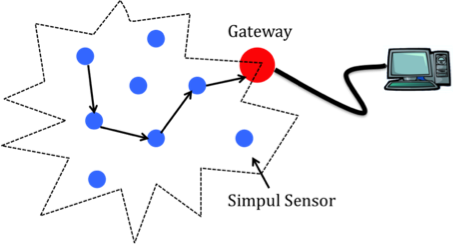
\includegraphics{gambar/wsn}
          \caption{Jaringan sensor nirkabel.}
          \label{wsn}
      \end{figure}

      \begin{figure}[H]
        \centering
          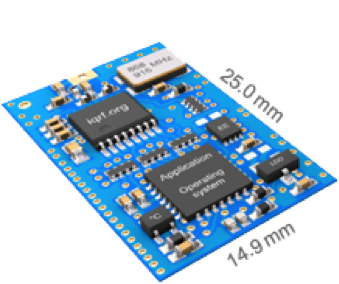
\includegraphics{gambar/iqrf}
          \caption{Contoh sebuah simpul sensor IQRF.}
          \label{iqrf}
      \end{figure}

    Pada umumnya, WSN adalah jaringan yang berdiri sendiri. Untuk menghubungkan WSN dengan jaringan yang lain misalnya jaringan internet, maka salah satu cara adalah dengan membangun \emph{gateway} WSN yang mampu menjembatani perbedaan protokol yang ada pada WSN dan jaringan internet. Cara tersebut adalah cara yang ditempuh dalam penelitian ini karena lebih mudah dilakukan dibandingkan dengan cara yang lain seperti sudah dijelaskan pada Bab Tinjauan Pustaka.

    Sementara itu, jaringan WiFi sebagai jaringan lokal nirkabel yang digunakan untuk komunikasi data dalam suatu area lokal dan sudah tersebar di berbagai tempat. Lokal yang dimaksud disini adalah area yang tidak terlalu luas yaitu dengan radius sekitar 20m atau dalam sebuah gedung. Untuk membangun jaringan lokal menggunakan WiFi, perangkat utama yang digunakan adalah AP. AP adalah piranti yang akan menjadi koordinator dalam jaringan lokal jika diinginkan topologi bintang (\emph{star}) seperti diilustrasikan pada Gambar \ref{star}.

      \begin{figure}[ht!]
        \centering
          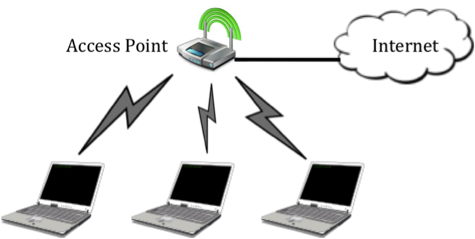
\includegraphics{gambar/star}
          \caption{Jaringan bintang menggunakan WiFi.}
          \label{star}
      \end{figure}

    Gambar \ref{star} memberi ilustrasi sebuah jaringan WiFi yang terdiri dari tiga buah komputer dan satu buah AP yang terhubung ke jaringan internet. Dengan konfigurasi tersebut, semua komputer yang ada di dalam jaringan WiFi dapat berkomunikasi dengan internet dengan aturan yang ditentukan oleh AP.

    Jika dilihat lebih dalam lagi, AP ini sebenarnya adalah piranti tertanam (\emph{embedded device}) yang didalamnya sudah terdapat pusat pengolahan utama, memori, dan penyimpanan (\emph{storage}). Dengan kenyataan inilah maka AP mempunyai potensi untuk menjagi \emph{gateway} bagi jaringan WiFi (IP) dan WSN ke jaringan internet. Untuk mengembangkan aplikasi yang akan ditanamkan ke dalam AP, maka diperlukan sistem operasi yang sesuai untuk AP. Karena pada dasarnya sistem Operasi dari pabrikan yang sudah tertanam pada AP tidak dapat dimodifikasi dan dikonfigurasi secara mudah. Oleh karena itu, sistem operasi harus diganti dengan sistem operasi baru yang dapat dikustomisasi dengan mudah.

  \subsection{IQRF}
    IQRF adalah teknologi komunikasi nirkabel berbasis paket melalui frekuensi radio dalam pita frekuensi sub-GHz \cite{MICRORISCs.r.o.2013,Sulc2011}. Teknologi ini dimaksudkan untuk penggunaan umum saat konektivitas nirkabel dibutuhkan, entah \emph{point to point} atau jaringan yang kompleks. Fungsionalitas lengkapnya bergantung semata-mata pada aplikasi berbahasa C yang ditulis oleh pengguna.

    Piranti komunikasi dasar dari IQRF adalah sebuah modul pancar-rima (\emph{transceiver}), termasuk unit mikrokontroller dengan sistem operasi tertanam yang mengimplementasikan lapisan \emph{link} dan lapisan jaringan (\emph{network layer}) yang mendukung jaringan jala (\emph{mesh network}). Tidak ada tingkat komunikasi yang lebih tinggi seperti lapisan \emph{transport} yang termasuk kedalam teknologi ini.

    Protokol jaringan jala dari piranti IQRF adalah IQMESH (\cite{Seflova2012}). IQMESH menggunakan koordinator jaringan untuk mengendalikan keseluruhan komunikasi. Sebuah jaringan IQMESH dapat menampung hingga 65.000 sensor. Setiap sensor di dalam jaringan memiliki alamat yang unik (\emph{logical address}) yang diberikan pada saat \emph{bonding}. Algoritma perutean \emph{Discovered Full Mesh} (DFM) memanfaatkan \emph{Virtual Routing Structure} (VRS) yang dibentuk pada saat proses \emph{discovery}.

    Fitur-fitur yang dimiliki antara lain:
      \begin{itemize}
        \item Kecepatan, daya, dan ukuran data yang rendah,
        \item RF yang berbasis paket data, maksimal 128 Byte per paket,
        \item pita frekuensi sub-GHz (868 MHz, 916 MHz, dst.), \emph{multichannel}, dan modulasi FSK,
        \item \emph{bit rate} 1.2 kb/s - 86.2 kb/s,
        \item daya keluaran maksimal 20 mW,
        \item maksimal 65.000 piranti dalam satu jaringan,
        \item konsumsi daya yang rendah: 380 nA saat \emph{standby}, 25 $\mu$A saat menerima.
      \end{itemize}


  \subsection{XBee}
    XBee adalah sebuah merk dari Digi International untuk keluarga modul radio \cite{DigiInternationalInc.2013}. XBee pertama diperkenalkan dalam merk MaxStream pada tahun 2005 yang berdasarkan pada standar IEEE 802.15.4-2003 untuk \emph{point to point} dan komunikasi bintang dalam \emph{baud rate} 250 kbit/s.

    Pada awalnya diperkenalkan dua model, yaitu 1mW XBee dan 100mW XBee-PRO. Sejak pertama kali diperkenalkan, beberapa buah XBee baru juga diperkenalkan dan semua XBee sekarang dipasarkan dengan merk Digi. Contoh piranti XBee dapat dilihat pada Gambar \ref{xbee}.

      \begin{figure}[H]
        \centering
          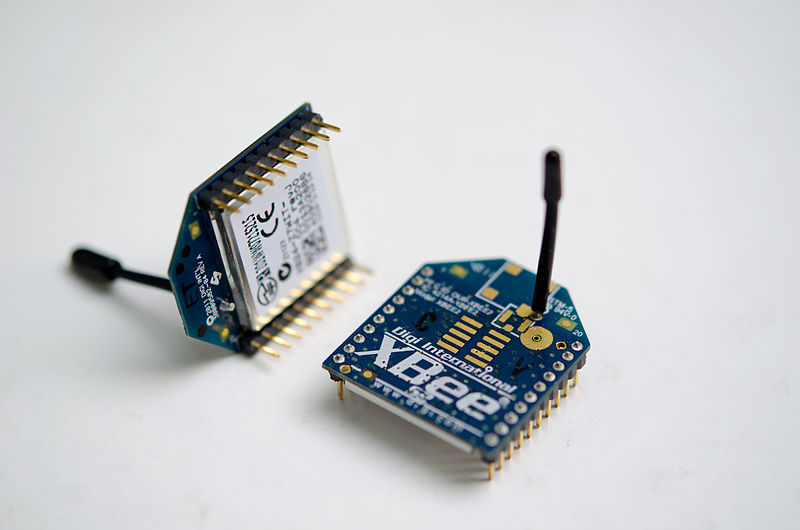
\includegraphics[width=0.5\textwidth]{gambar/xbee}
          \caption{Sepasang piranti XBee.}
          \label{xbee}
      \end{figure}

    Pada Gambar \ref{xbee} dapat dilihat dua buah XBee radio yang tidak tertanam pada piranti lain. XBee radio memiliki 20 kaki (\emph{pin}) yang dapat ditancapkan pada piranti lain.

  \subsection{TCP/IP}
    Protokol internet adalah kumpulan protokol-protokol komunikasi yang digunakan dalam internet dan jaringan komputer sejenis, dan umumnya merupakan protokol yang paling populer untuk WAN. Pada umumnya hal ini dikenal dengan TCP/IP, karena protokol utamanya merupakan protokol jaringan pertama yang terstandarisasi. Terkadang hal ini dikenal dengan model DoD karena pengaruh ARPANET pada dekade 1970an.

    TCP/IP menyediakan konektivitas antar ujung yang menspesifikasikan bagaimana data harus diformat, dialamatkan, ditransmisikan, dirutekan, dan diterima di tujuan. TCP/IP memiliki empat layer abstraksi yang digunakan untuk mengurutkan semua protokol internet menurut jangkauan jaringan yang terlibat. Dari terendah sampai tertinggi, lapisan-lapisan tersebut adalah layer link, layer internet, layer transport, dan layer aplikasi.

  \subsection{\emph{Access Point}}
    \emph{Access Point}, disingkat AP, atau juga dikenal dengan istilah \emph{Wireless Access Point} adalah sebuah piranti yang memungkinkan piranti-piranti nirkabel untuk terkoneksi dengan jaringan kabel menggunakan Wi-Fi atau standar lain. AP biasanya terkoneksi dengan sebuah \emph{router} (melalui jaringan kabel) sebagai piranti yang berdiri sendiri, namun juga dapat menjadi bagian dalam komponen \emph{router} tersebut.

    Penggunaan secara korporat melibatkan beberapa AP ke dalam jaringan kabel dan menyediakan akses nirkabel ke LAN kantor. AP diatur dengan WLAN \emph{Controller} yang menangani pengaturan daya RF, kanal-kanal, autentikasi, dan keamanan.
    
    Sebuah \emph{hotspot} adalah aplikasi dari satu atau beberapa AP, yang memungkinkan piranti dapat terhubung ke Internet dengan mudah. Konsep ini sudah menjadi hal yang umum di beberapa kota besar. Kombinasi dari warung kopi, perpustakaan, dan AP milik pribadi memungkinkan klien untuk terkoneksi dengan Internet. Koleksi dari \emph{hotspot} yang terkoneksi dapat disebut sebagai sebuah jaringan \emph{lily pad}.

  \subsection{TP-LINK MR3020}
    TP-LINK MR3020 adalah \emph{Portable 3G/4G Wireless N Router} keluaran TP-LINK, perusahaan asal Shenzen, China, yang bergerak dalam bidang piranti jaringan komputer. TP-LINK MR3020 pada dasarnya adalah Wi-Fi router yang dapat meneruskan internet dari modem 3G/4G yang terpasang di port USB-nya. TP-LINK MR3020 termasuk AP yang populer karena bentuknya yang kecil, seperti dapat dilihat pada Gambar \ref{mr3020}, sehingga mudah dibawa dan harganya yang tergolong murah. Banyak forum di internet yang membahas AP jenis ini, sehingga dukungan untuk memanipulasinya luas dari komunitas. Penelitian ini menggunakan sistem operasi OpenWRT guna memberikan fleksibilitas dalam pengembangan aplikasi \emph{gateway} berbasis web.

    \begin{figure}[H]
      \centering
        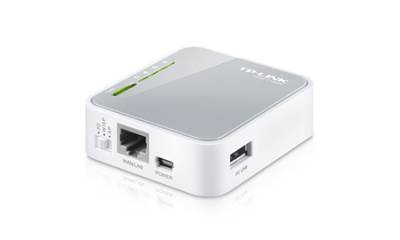
\includegraphics[width=10cm]{gambar/mr3020}
        \caption{TP-LINK MR3020.}
        \label{mr3020}
    \end{figure}

    Seperti yang tampak pada Gambar \ref{mr3020}, TP-LINK MR3020 memiliki satu buah \emph{port} USB dan satu buah \emph{port} RJ-45. Untuk sumber daya listrik, AP ini menggunakan koneksi \emph{micro}-USB.

    Spesifikasi teknis dari fitur perangkat keras dan komunikasi nirkabel dari MR3020 dapat dilihat pada Tabel \ref{mr3020-hardware-feature} dan Tabel \ref{mr3020-wireless-feature}.

    \begin{table}[H]
    \centering
    \caption{Fitur perangkat keras dari TP-LINK MR3020.}
    \label{mr3020-hardware-feature}
    \begin{tabular}{|l|p{10cm}|}
    \hline
    \multicolumn{2}{|c|}{Fitur Perangkat Keras}                                                                                                \\ \hline
    Antarmuka             & 1 10/100Mbps WAN/LAN Port, USB 2.0 Port for 3G/4G modem, a mini USB Port for power supply.   \\ \hline
    Tombol                & Quick Setup Security Button, Reset Button, Mode Switch                                                             \\ \hline
    Suplai Daya Eksternal & 5VDC/1.0A                                                                                                          \\ \hline
    Dimensi (P x L xT)    & 2.9 x 2.6 x 0.9 in. (74 x 67 x22 mm)                                                                               \\ \hline
    Tipe Antena           & Internal Antenna                                                                                                   \\ \hline
    \end{tabular}
    \end{table}

    \begin{table}[H]
    \centering
    \caption{Fitur komunikasi nirkabel dari TP-LINK MR3020.}
    \label{mr3020-wireless-feature}
    \begin{tabular}{|l|p{10cm}|}
    \hline
    \multicolumn{2}{|c|}{Fitur Komunikasi Nirkabel}                                         \\ \hline
    Standar Nirkabel   & IEEE 802.11n, IEEE 802.11g, IEEE 802.11b                           \\ \hline
    Frekuensi          & 2.4-2.4835GHz                                                      \\ \hline
    EIRP               & <20dBm                                                             \\ \hline
    Mode Nirkabel      & 3G Router, Travel Router (AP), WISP Client Router                  \\ \hline
    Sekuritas Nirkabel & Support 64/128 bit WEP, WPA-PSK/WPA2-PSK, Wireless MAC Filtering   \\ \hline
    \end{tabular}
    \end{table}

  \subsection{Web Server}
    Web server dapat mengacu pada perangkat keras atau perangkat lunak yang membantu dalam penyampaian konten web yang dapat diakses melalui internet.

    Penggunaan web server yang paling umum adalah sebagai host untuk halaman web, walaupun ada beberapa penggunaan lain seperti game, media penyimpan data, atau penjalanan aplikasi perusahaan.

    Pemilihan aplikasi yang bertindak sebagai Web Server pada piranti tertanam (\emph{embedded device}) harus mempertimbangkan spesifikasi dari piranti tersebut. Penggunaan aplikasi Web Server yang biasa ditanamkan pada komputer \emph{desktop} bahkan \emph{server}, misal Apache, sangat tidak tepat bila ditanamkan pada piranti tertanam. Hal ini akan mengakibatkan pemborosan pada penggunaan sumber daya karena piranti tertanam memiliki sumber daya yang sangat terbatas. Piranti tertanam sebaiknya menggunakan aplikasi web server yang dirancang secara spesifik untuk piranti tersebut. Pilihan yang ada antara lain uhttpd dan light-httpd.


  \subsection{\emph{Asynchronous JavaScript and XML}}
    \emph{Asynchronous JavaScript and XML}, atau lebih populer dengan istilah AJAX, adalah kelompok dari teknik-teknik pengembangan web yang digunakan pada klien untuk membuat aplikasi asinkron. Dengan AJAX, aplikasi web dapat mengirim dan menerima data dari sebuah server secara asinkron tanpa mengganggu tampilan dari halaman yang ada. Data dapat diambil menggunakan obyek XMLHttpRequest.

    AJAX bukanlah sebuah teknologi, tapi kelompok dari beberapa teknologi. HTML dan CSS dapat digunakan dalam kombinasi untuk menyajikan informasi yang akan ditampilkan. Kemudian, DOM diakses oleh JavaScript untuk menampilkan dan mengijinkan pengguna untuk berinteraksi dengan informasi tertampil. JavaScript dan obyek XMLHttpRequest menyediakan sebuah metode pertukaran data secara asinkron antara \emph{browser} dan \emph{server} untuk menghindari proses muat ulang halaman secara keseluruhan.


  \subsection{OpenWRT}
    OpenWRT adalah sebuah sistem operasi untuk \emph{embedded device} yang berbasis pada Linux kernel \cite{OpenWrtProject2013}. OpenWRT pada umumnya digunakan dalam routing \emph{network traffic}. Komponen-komponen utamanya adalah Linux kernel, util-linux, uClibc dan BusyBox. Semua komponen sudah dioptimalkan dan dimampatkan untuk bisa dimuat dalam \emph{router} rumahan yang memiliki keterbatasan media penyimpan dan memori. OpenWRT dapat dikonfigurasikan melalui antarmuka \emph{command-line} (\emph{ash shell}), seperti dapat dilihat pada Gambar \ref{openwrt}, atau dengan antarmuka Web (LuCI). Terdapat kurang lebih 3.500 paket-paket perangkat lunak tambahan yang tersedia untuk diinstal melalui sistem manajemen paket \emph{opkg}.

      \begin{figure}[ht!]
        \centering
          
\includegraphics[width=10cm]{gambar/openwrt}
          \caption{Tampilan antarmuka \emph{command-line} OpenWRT versi \emph{BackFire}.}
          \label{openwrt}
      \end{figure}

    OpenWRT dapat berjalan pada router CPE (\emph{Customer Premised Equipment}), \emph{gateway} residensial, komputer saku (seperti Ben NanoNote), dan komputer jinjing. OpenWRT juga dapat berjalan pada komputer konvensional atau komputer dengan arsitektur x86. Banyak \emph{patch} dari kode sesumber berbasis OpenWRT yang diubah ke dalam Linux kernel utama.

  \subsection{SSHFS}
    SSHFS (SSH Filesystem) adalah sebuah klien \emph{filesystem} untuk \emph{mount} dan berinteraksi dengan direktori dan arsip yang berlokasi pada server atau \emph{workstation}. Klien berinteraksi dengan server dengan SSH \emph{File Transfer Protocol} (SFTP), sebuah protokol jaringan yang menyediakan akses ke arsip, transfer arsip, dan fungsionalitas manajemen arsip melalui aliran data yang didesain sebagai ekstensi dari protokol SSH versi 2.0.

  \subsection{Bootstrap}
    Bootstrap adalah koleksi gratis dari alat-alat untuk membuat situs web dan aplikasi berbasis web. Bootstrap terdiri dari HTML dan contoh desain berbasis CSS untuk tipografi, borang, tombol, navigasi, komponen antarmuka lain, dan juga ekstensi JavaScript yang bersifat opsional.

    Bootstrap merupakan proyek paling populer pada GitHub, dan sudah digunakan oleh, diantaranya, NASA dan MSNBC.

  \subsection{Sublime Text 3}
    Sublime Text adalah aplikasi teks editor \emph{cross-platform} yang memiliki \emph{Application Programming Interface} (API) Python. Sublime Text juga dapat menambah fungsionalitasnya dengan beberapa tambahan \emph{plugin}. Aplikasi ini bukan merupakan aplikasi \emph{open source} atau aplikasi gratis. Versi 3 dari Sublime Text dirilis dalam versi beta pada 29 Januari 2013. Antar muka Sublime Text dapat dilihat pada Gambar \ref{sublime-text}.

      \begin{figure}[ht!]
        \centering
          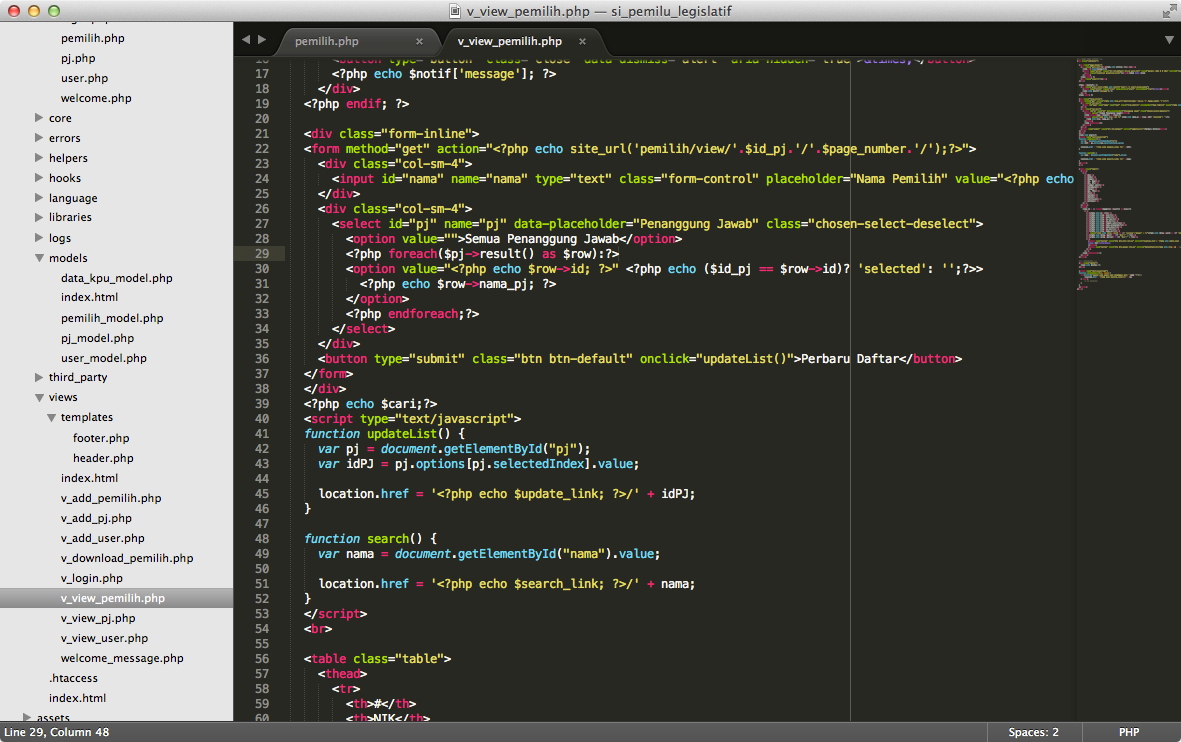
\includegraphics[width=0.9\textwidth]{gambar/sublime-text}
          \caption{Aplikasi Sublime Text 3 yang berjalan pada Mac OS X.}
          \label{sublime-text}
      \end{figure}
    
    Antar muka Sublime Text sangat sederhana. Antar muka terdiri atas \emph{side bar} yang menampilkan direktori \emph{project} yang sedang dikerjakan pada sebelah kiri dan teks editor pada sebelah kanan.

    Sublime Text mendukung beberapa bahasa pemrograman dan mampu memberikan warna-warna pada kode tertentu (\emph{syntax highlighting}) untuk mempermudah penulisan kode. Bahasa yang didukung antara lain ActionScript, AppleScript, ASP, batch files, C, C$++$, C\#,Clojure, CSS, D, Diff, Erlang, Go, Graphviz (DOT), Groovy, Haskell, HTML, Java, JSP, JavaScript, JSON, LaTeX, Lisp, Lua, Makefiles, Markdown, MATLAB, Objective-C, OCaml, Perl, PHP, Python, R, Rails, Regular Expressions, reStructuredText, Ruby, Scala, shell scripts (Bash), SQL, Tcl, Textile, XML, XSL, dan YAML. Sublime Text juga dapat menambahkan dukungan \emph{syntax highlighting} pada bahasa pemrograman lain dengan tambahan \emph{plugin}.

% Baris ini digunakan untuk membantu dalam melakukan sitasi
% Karena diapit dengan comment, maka baris ini akan diabaikan
% oleh compiler LaTeX.
\begin{comment}
\bibliography{daftar-pustaka}
\end{comment}
